\documentclass{beamer}
\usepackage[utf8]{inputenc}

\usetheme{Madrid}
\usecolortheme{default}
\usepackage{amsmath,amssymb,amsfonts,amsthm}
\usepackage{txfonts}
\usepackage{tkz-euclide}
\usepackage{listings}
\usepackage{adjustbox}
\usepackage{array}
\usepackage{tabularx}
\usepackage{gvv}
\usepackage{lmodern}
\usepackage{circuitikz}
\usepackage{tikz}
\usepackage{graphicx}

\setbeamertemplate{page number in head/foot}[totalframenumber]

\usepackage{tcolorbox}
\tcbuselibrary{minted,breakable,xparse,skins}



\definecolor{bg}{gray}{0.95}
\DeclareTCBListing{mintedbox}{O{}m!O{}}{%
  breakable=true,
  listing engine=minted,
  listing only,
  minted language=#2,
  minted style=default,
  minted options={%
    linenos,
    gobble=0,
    breaklines=true,
    breakafter=,,
    fontsize=\small,
    numbersep=8pt,
    #1},
  boxsep=0pt,
  left skip=0pt,
  right skip=0pt,
  left=25pt,
  right=0pt,
  top=3pt,
  bottom=3pt,
  arc=5pt,
  leftrule=0pt,
  rightrule=0pt,
  bottomrule=2pt,
  toprule=2pt,
  colback=bg,
  colframe=orange!70,
  enhanced,
  overlay={%
    \begin{tcbclipinterior}
    \fill[orange!20!white] (frame.south west) rectangle ([xshift=20pt]frame.north west);
    \end{tcbclipinterior}},
  #3,
}
\lstset{
    language=C,
    basicstyle=\ttfamily\small,
    keywordstyle=\color{blue},
    stringstyle=\color{orange},
    commentstyle=\color{green!60!black},
    numbers=left,
    numberstyle=\tiny\color{gray},
    breaklines=true,
    showstringspaces=false,
}
\begin{document}

\title 
{5.2.36}
\date{September 11,2025}


\author 
{Kavin B-EE25BTECH11033}






\frame{\titlepage}
\begin{frame}{Question}
Solve the following system of linear equations.
\begin{align*}
    3x-5y-4=0
\end{align*}
\begin{align*}
    9x=2y+7
\end{align*}
\bigskip
\end{frame}



\begin{frame}{Theoretical Solution}

The equation of line $L_1$ is,
\begin{align}
    \myvec{3 & -5}\vec{x} = 4
\end{align}
The equation of line $L_2$ is,
\begin{align}
    \myvec{9 & -2}\vec{x} = 7
\end{align}
On putting the equations in a matrix, we will get
\begin{align}
    \implies \myvec{3 & -5\\9 & -2}\vec{x} = \myvec{4\\7}
\end{align}
\end{frame}

\begin{frame}{Theoretical Solution}
So the augmented matrix is,
\begin{align}
    \augvec{2}{1}{3 & -5 & 4\\9 & -2 & 7}
\end{align}
\begin{align}
    R_2\rightarrow R_2-3R_1\implies\augvec{2}{1}{3 & -5 & 4\\0 & 13 & -5}
\end{align}
\begin{align}
    R_2\rightarrow \frac{1}{13}R_2\implies\augvec{2}{1}{3 & -5 & 4\\0 & 1 & -5/13}
\end{align}
\begin{align}
    R_1\rightarrow R_1+5R_2\implies\augvec{2}{1}{3 & 0 & 27/13\\0 & 1 & -5/13}
\end{align}
\end{frame}


\begin{frame}{Theoretical Solution}
\begin{align}
    R_1\rightarrow \frac{1}{3}R_1\implies\augvec{2}{1}{1 & 0 & 9/13\\0 & 1 & -5/13}
\end{align}
\begin{align}
    \implies\vec{x} =\myvec{x\\y}\equiv \myvec{9/13\\-5/13}
\end{align}
Therefore the two lines will intersect at \myvec{9/13\\-5/13}.
\end{frame}

\begin{frame}{Plot}
    \centering
    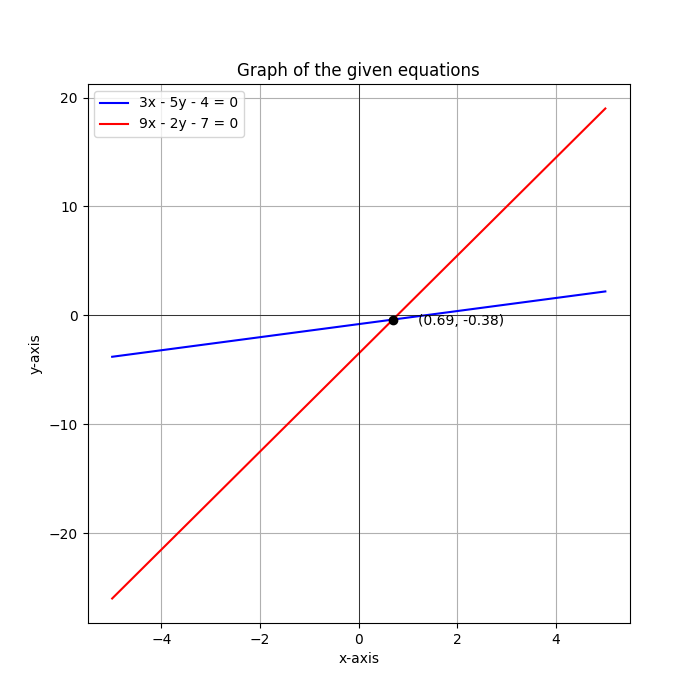
\includegraphics[width=\columnwidth, height=0.8\textheight, keepaspectratio]{figs/fig.png}
\end{frame}


\end{document}
